\documentclass[12pt, a4paper]{article}
\usepackage{../../../myconfig} % Gọi file cấu hình từ ngoài gốc vào

% ==========================================
% BẮT ĐẦU NỘI DUNG TÀI LIỆU
% ==========================================
\begin{document}

% Truyền 3 tham số: {Nhãn cam} {Chữ to chính giữa} {Chữ ở góc phải Header}
\titlebox{Chủ đề: Hàm số}{Cực trị của hàm số}{Hàm số: Cực trị}

\begin{center}
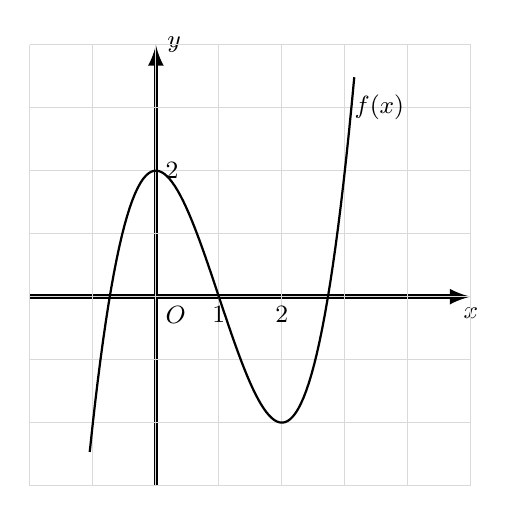
\begin{tikzpicture}[>=latex, scale=0.8]
    % Hệ trục tọa độ
    \draw[->, ultra thick] (-2,0) -- (5,0) node[below] {\small $x$};
    \draw[->, ultra thick] (0,-3) -- (0,4) node[right] {\small $y$};
    \node[below right] at (0,0) {\small $O$};
    \foreach \x in {-1,1,2,3} {
         \draw (\x,0.05) -- (\x,-0.05) ;
    }
    \foreach \y in {-2,-1,1,2,3} {
          \draw (0.05,\y) -- (-0.05,\y)   ;
    }
    \draw[color=gray!30, thin, step=1] (-2,-3) grid (5,4);
    % Đồ thị hàm bậc 3: y = -x^3 + 3x^2 + 2
    \draw[thick, samples=100, domain=-1.05:3.15] 
        plot (\x, {\x*\x*\x - 3*\x*\x + 2});
    \node[right] at (3,3) {\small $f(x)$};
    \node [below] at (1,0) {\small $1$};
   \node [below] at (2,0) {\small $2$};
   \node [right] at (0,2) {\small $2$};
\end{tikzpicture}

\end{center}
\drawdashlines{20}
\newpage

\questionLinesManual{5}{1}{Cho hàm số \( y = f(x) \) có đồ thị như hình vẽ. Điểm cực tiểu của đồ thị hàm số đã cho là
\begin{center}
\begin{tikzpicture}[>=latex, scale=0.8]
    % Hệ trục tọa độ
    \draw[->] (-2.5,0) -- (3.5,0) node[below] {$x$};
    \draw[->] (0,-5) -- (0,2) node[right] {$y$};
    \node[above left] at (0,0) {$O$};
    
    % Đánh dấu các điểm
    \node[above] at (-1,0) {$-1$};
    \node[above] at (1,0) {$1$};
    \node[above right] at (2,0) {$2$};
    \node[left] at (0,-4) {$-4$};
    \node[left] at (0,-2) {$-2$};
    
    % Vẽ đồ thị hàm số y = x^3 - 3x^2 - 4x + 6
    \draw[thick, color=black!80, samples=150, domain=-1.65:2.1] 
        plot (\x, {\x*\x*\x - 3*\x - 2});
    
    % Đường nét đứt
    \draw[dashed] (1,0) -- (1,-4) -- (0,-4);
\end{tikzpicture}
\end{center}}

\questionLinesManual{5}{2}{Cho hàm số \( y = ax^3 + bx^2 + cx + d \) (\( a, b, c, d \in \mathbb{R} \)) có đồ thị như hình vẽ bên. Số điểm cực trị của hàm số này là
\begin{center}
\begin{tikzpicture}[>=latex, scale=0.8]
    % Hệ trục tọa độ
    \draw[->] (-3.5,0) -- (3.5,0) node[below] {$x$};
    \draw[->] (0,-3.5) -- (0,3.5) node[right] {$y$};
    \node[above left] at (0,0) {$O$};
    
    
    % Vẽ đồ thị hàm bậc 3 y = x^3 - 3x
    \draw[thick, color=black!80, samples=150, domain=-2.1:2.1] 
        plot (\x, {\x*\x*\x - 3*\x});
    
\end{tikzpicture}
\end{center}}{%
\begin{tasks}(4)
\task 3
\task 2
\task 0
\task 1
\end{tasks}
}

\questionLinesManual{5}{3}{Cho hàm số \( y = f(x) \) có đồ thị như hình vẽ
\begin{center}
\begin{tikzpicture}[>=latex, scale=0.8]
    % Hệ trục tọa độ
    \draw[->] (-3.5,0) -- (3.5,0) node[below] {$x$};
    \draw[->] (0,-3.5) -- (0,3.5) node[right] {$y$};
    \node[above left] at (0,0) {$O$};
    
    % Đánh dấu các điểm trên trục
    \node[below] at (-1,0) {$-1$};
    \node[below] at (1,0) {$1$};
    \node[right] at (0,-2) {$-2$};
    \node[left] at (0,2) {$2$};
    
    % Vẽ đồ thị hàm số bậc 3 y = x^3 - 3x
    \draw[thick, color=black!80, samples=150, domain=-3:-0.3] 
       plot (\x, {(\x*\x + 1)/\x});
    \draw[thick, color=black!80, samples=150, domain=0.3:3] 
       plot (\x, {(\x*\x + 1)/\x});
    % Đường nét đứt
    \draw[dashed] (-1,0) -- (-1,-2) -- (0,-2);
    \draw[dashed] (1,0) -- (1,2)-- (0,2);
\end{tikzpicture}
\end{center}
Giá trị cực tiểu của hàm số đã cho là}

\questionLinesManual{5}{4}{Cho hàm số \( y = f(x) \) liên tục trên \( \mathbb{R} \) và có đồ thị như hình dưới đây.
\begin{center}
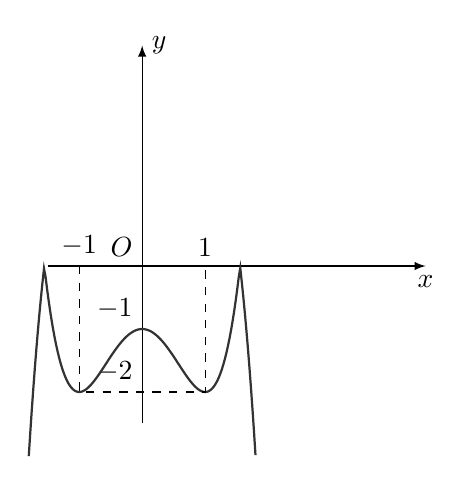
\begin{tikzpicture}[>=latex, scale=0.8]
    % Hệ trục tọa độ
    \draw[->] (-1.5,0) -- (4.5,0) node[below] {$x$};
    \draw[->] (0,-2.5) -- (0,3.5) node[right] {$y$};
    \node[above left] at (0,0) {$O$};
    
    % Đánh dấu các điểm trên trục
    \node[above] at (1,0) {$1$};
    \node[above] at (-1,0) {$-1$};
    \node[above left] at (0,-1) {$-1$};
    \node[above left] at (0,-2) {$-2$};
    
    % Vẽ đồ thị hàm bậc 4
    \draw[thick, color=black!80, samples=150, domain=-1.8:1.8] 
       plot (\x, {-abs(\x*\x*\x*\x - 2*\x*\x - 1)});
    % Đường nét đứt
    \draw[dashed] (-1,0) -- (-1,-2) -- (1,-2) -- (1,0);
\end{tikzpicture}
\end{center}
Hàm số đã cho có bao nhiêu điểm cực đại?}

\newpage
\drawdashlines{35}
\newpage

\questionLinesManual{10}{5}{Đồ thị hàm số \( y = x^3 - 6x^2 + 9x - 1 \) có toạ độ điểm cực đại là}

\questionLinesManual{10}{6}{Số điểm cực tiểu của hàm số \( f(x) = x^4 - x^2 + 2 \) là}

\questionLinesManual{10}{7}{Hàm số \( y = \dfrac{2x + 3}{x + 1} \) có bao nhiêu điểm cực trị?}

\questionLinesManual{10}{8}{Cho hàm số \( y = \dfrac{x^2 + 3}{x + 1} \). Mệnh đề nào dưới đây đúng?}

\questionLinesManual{4}{9}{Cho hàm số bậc ba \( y = f(x) \) có bảng biến thiên như sau:
\begin{center}

\begin{tikzpicture}[>=stealth]
    \tkzTabInit[nocadre=false,lgt=1.2,espcl=2.5]
    {$x$ / 1, $f'(x)$ / 1, $f(x)$ / 2.5}
    {$-\infty$, $-1$, $1$, $+\infty$}
    \tkzTabLine{ , +, 0, -, 0, + }
    \tkzTabVar{-/$-\infty$, +/$4$, -/$0$, +/$+\infty$}

\end{tikzpicture}
\end{center}
Điểm cực tiểu của đồ thị hàm số là:}

\questionLinesManual{4}{10}{Cho hàm số \( y = f(x) = \dfrac{mx^2 + nx + p}{qx + r} \) có bảng biến thiên như hình vẽ bên dưới.
\begin{center}

\begin{tikzpicture}[>=stealth]
    \tkzTabInit[nocadre=false,lgt=1.2,espcl=2]
    {$x$ / 1, $f'(x)$ / 1, $f(x)$ / 2.5}
    {$-\infty$, $-3$, $-1$, $1$, $+\infty$}
    \tkzTabLine{ , +, 0, -, d, -, 0, + }
    \tkzTabVar{-/$-\infty$, +/$5$,-D+/$-\infty$ /$+\infty$, -/$3$, +/$+\infty$}

\end{tikzpicture}
\end{center}
Giá trị cực đại của hàm số đã cho bằng}

\questionLinesManual{5}{11}{Cho hàm số \( y = f(x) \) có bảng biến thiên như sau:
\begin{center}

\begin{tikzpicture}[>=stealth]
    \tkzTabInit[nocadre=false,lgt=1.2,espcl=2]
    {$x$ / 1, $y'$ / 1, $y$ / 2.5}
    {$-\infty$, $-3$, $-2$, $1$, $+\infty$}
    \tkzTabLine{ , -, 0, +, d, +, 0, - }
    \tkzTabVar{+/$+\infty$, -/$5$,+D-/$+\infty$ /$-\infty$, +/$0$, -/$-\infty$}
\end{tikzpicture}
\end{center}
Giá trị cực đại của hàm số \( y = f(x) \) là:}


\questionLinesManual{5}{12}{Cho hàm số \( f(x) \) có bảng biến thiên như sau:
\begin{center}

\begin{tikzpicture}[>=stealth]
    \tkzTabInit[nocadre=false,lgt=1.2,espcl=2.5]
    {$x$ / 1, $f'(x)$ / 1}
    {$-\infty$, $-1$, $2$, $+\infty$}
    \tkzTabLine{ , +, 0, -, 0, + }
\end{tikzpicture}
\end{center}
Hàm số đã cho đạt cực đại tại}

\questionLinesManual{5}{13}{Cho hàm \( f(x) \) liên tục trên \( \mathbb{R} \) có bảng xét dấu như sau:
\begin{center}

\begin{tikzpicture}[>=stealth]
    \tkzTabInit[nocadre=false,lgt=1.2,espcl=2.5]
    {$x$ / 1, $f'(x)$ / 1}
    {$-\infty$, $0$, $3$, $+\infty$}
    \tkzTabLine{ , +, d, -, 0, + }
\end{tikzpicture}
\end{center}
Hàm số có bao nhiêu điểm cực trị}

\questionLinesManual{5}{14}{Cho hàm số \( f(x) \) liên tục trên \( \mathbb{R} \) có bảng xét dấu như sau:
\begin{center}

\begin{tikzpicture}[>=stealth]
    \tkzTabInit[nocadre=false,lgt=1.2,espcl=2.5]
    {$x$ / 1, $f'(x)$ / 1}
    {$-\infty$, $1$, $3$, $+\infty$}
    \tkzTabLine{ , +, d, -, 0, + }
\end{tikzpicture}
\end{center}
Hàm số có bao nhiêu điểm cực trị:}


% ====== CÂU 24 ======
\questionLinesManual{5}{15}{Cho hàm số \( f(x) \) xác đinh trên \(\mathbb{R} \setminus \{3\}\) có bảng xét dấu như sau:
\begin{center}

\begin{tikzpicture}[>=stealth]
    \tkzTabInit[nocadre=false,lgt=1.2,espcl=2.5]
    {$x$ / 1, $f'(x)$ / 1}
    {$-\infty$, $1$, $3$, $+\infty$}
    \tkzTabLine{ , -, 0, +, d, - }
\end{tikzpicture}
\end{center}
Hàm số có bao nhiêu điểm cực đại}

% ====== CÂU 25 ======
\questionLinesManual{5}{16}{Cho hàm số \( y = f(x) \) xác định trên \(\mathbb{R} \setminus \{1\}\) có bảng xét dấu như sau:
\begin{center}

\begin{tikzpicture}[>=stealth]
    \tkzTabInit[nocadre=false,lgt=1.2,espcl=2]
    {$x$ / 1, $y'$ / 1}
    {$-\infty$, $-1$, $0$, $1$, $+\infty$}
    \tkzTabLine{ , -, d, +, 0, -, d, + }
\end{tikzpicture}
\end{center}
Hàm số có bao nhiêu điểm cực trị}

\newpage
\drawdashlines{35}
\newpage

% ====== CÂU 61 ======
\questionLinesManual{7}{17}{Cho hàm số \( y = f(x) \) liên tục trên \( \mathbb{R} \) và có đạo hàm  
\( f'(x) = (x+1)^3(x-1)(x-2). \) 
Số điểm cực trị của hàm số đã cho là}

% ====== CÂU 62 ======
\questionLinesManual{7}{18}{Hàm số \( f(x) \) có đạo hàm  
\( f'(x) = x^2(x-1)(x-2)^3, \quad \forall x \in \mathbb{R}. \)  
Hàm số \( f(x) \) có bao nhiêu điểm cực đại?}

\questionLinesManual{7}{19}{Cho hàm số \( f(x) \) có đạo hàm  
\( f'(x) = x^2(x+2)(x^2+x-2)(x-1)^4 \)
với mọi \( x \in \mathbb{R} \). Số điểm cực trị của hàm số đã cho là}

\questionLinesManual{7}{20}{Cho hàm số \( f(x) \) có đạo hàm \( f'(x) = x(x-1)(x+2)^3 \), \( \forall x \in \mathbb{R} \). Số điểm cực trị của hàm số đã cho là}

\newpage

\begin{center}
    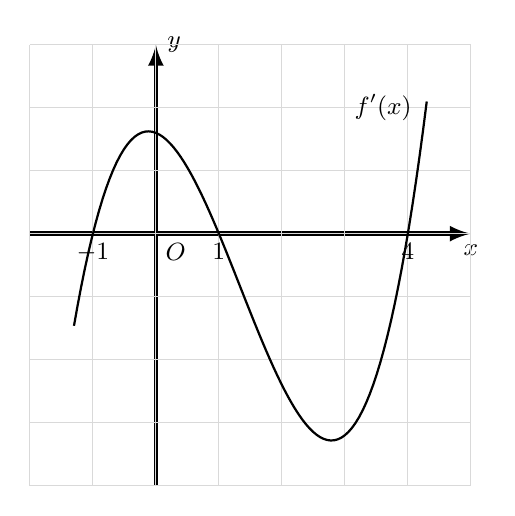
\begin{tikzpicture}[>=latex, scale=0.8]
    % Hệ trục tọa độ
    \draw[->, ultra thick] (-2,0) -- (5,0) node[below] {\small $x$};
    \draw[->, ultra thick] (0,-4) -- (0,3) node[right] {\small $y$};
    \node[below right] at (0,0) {\small $O$};
    \foreach \x in {-1,1,2,3} {
         \draw (\x,0.05) -- (\x,-0.05) ;
    }
    \foreach \y in {-2,-1,1,2,3} {
          \draw (0.05,\y) -- (-0.05,\y)   ;
    }
    \draw[color=gray!30, thin, step=1] (-2,-4) grid (5,3);
    % Đồ thị hàm bậc 3: y = -x^3 + 3x^2 + 2
    \draw[thick, samples=100, domain=-1.3:4.3] 
        plot (\x, {0.4*(\x+1)*(\x-1)*(\x-4)});
    \node[right] at (3,2) {\small $f'(x)$};
   \node [below] at (1,0) {\small $1$};
   \node [below] at (4,0) {\small $4$};
   \node [below] at (-1,0) {\small $-1$};
\end{tikzpicture}
\end{center}
\drawdashlines{25}
\newpage

\questionLinesManual{8}{21}{Cho hàm đa thức \( y = f(x) \). Đồ thị hàm số \( y = f'(x) \) là đường cong như hình vẽ bên dưới. Hỏi hàm số \( y = f(x) \) có bao nhiêu điểm cực trị?
\begin{center}
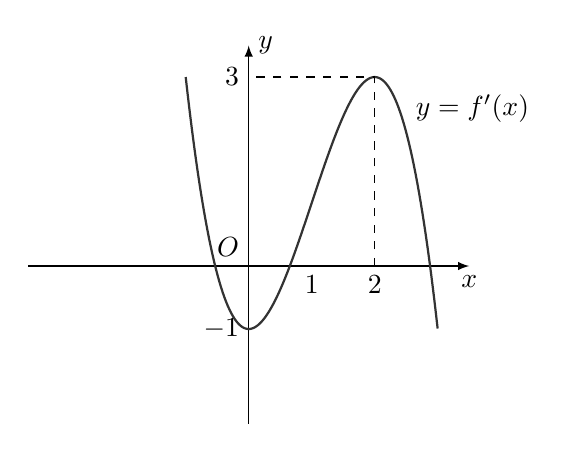
\begin{tikzpicture}[>=latex, scale=0.8]
    % Hệ trục tọa độ
    \draw[->] (-3.5,0) -- (3.5,0) node[below] {$x$};
    \draw[->] (0,-2.5) -- (0,3.5) node[right] {$y$};
    \node[above left] at (0,0) {$O$};
    
    % Đánh dấu các điểm
    \node[left] at (0,-1) {$-1$};
    \node[below] at (1,0) {$1$};
    \node[below] at (2,0) {$2$};
    \node[left] at (0,3) {$3$};
    
    % Vẽ đồ thị f'(x)
    \draw[thick, color=black!80, samples=150, domain=-1:3] 
       plot (\x, {-\x*\x*\x + 3*\x*\x - 1});
    \draw[dashed] (2,0) -- (2,3) -- (0,3);
    \node[right] at (2.5,2.5) {$y = f'(x)$};
\end{tikzpicture}
\end{center}}

% ====== CÂU 87 ======
\questionLinesManual{8}{22}{Cho hàm số \( y = f(x) \) có đạo hàm trên \( \mathbb{R} \). Biết hàm số \( y = f'(x) \) có đồ thị như hình vẽ. Phát biểu nào sau đây là đúng?
\begin{center}
\begin{tikzpicture}[>=latex, scale=0.8]
    % Hệ trục tọa độ
    \draw[->] (-3.5,0) -- (3.5,0) node[below] {$x$};
    \draw[->] (0,-2) -- (0,3.5) node[right] {$y$};
    \node[above left] at (0,0) {$O$};
    
    % Đánh dấu các điểm
    \node[below] at (-2,0) {$-2$};
    \node[below] at (1,0) {$1$};
    \node[right] at (0,2) {$2$};
    
    % Vẽ đồ thị f'(x) là parabol hướng xuống có nghiệm tại x = -2 và x = 1
    \draw[thick, color=black!80, samples=150, domain=-2.3:1.3] 
        plot (\x, {-(\x+2)*(\x-1)});
    
    \node[right] at (1.5,2) {$y = f'(x)$};
\end{tikzpicture}
\end{center}
Điểm cực đại của đồ thị hàm số f(x) là}


\end{document}